\documentclass[tikz,border=5pt]{standalone}
\usepackage{pgfplots}
\pgfplotsset{compat=1.18}
\usepackage{fontspec}
\setsansfont{SourceSansPro}[
  Path = /usr/local/texlive/2024/texmf-dist/fonts/opentype/adobe/sourcesanspro/,
  UprightFont = SourceSansPro-Regular.otf,
  BoldFont = SourceSansPro-Bold.otf,
  ItalicFont = SourceSansPro-RegularIt.otf,
  BoldItalicFont = SourceSansPro-BoldIt.otf,
  Scale = 1.0
]
\usetikzlibrary{positioning}
\usepackage{xcolor}
\definecolor{primaryblue}{HTML}{012169}
\definecolor{primarygold}{HTML}{B9975B}
\definecolor{highlightyellow}{HTML}{F2A900}
\definecolor{lightbg}{HTML}{E8EDF5}
\definecolor{jet}{HTML}{1A1A1A}
\definecolor{positivegreen}{HTML}{15803D}
\definecolor{negativered}{HTML}{B91C1C}
\begin{document}
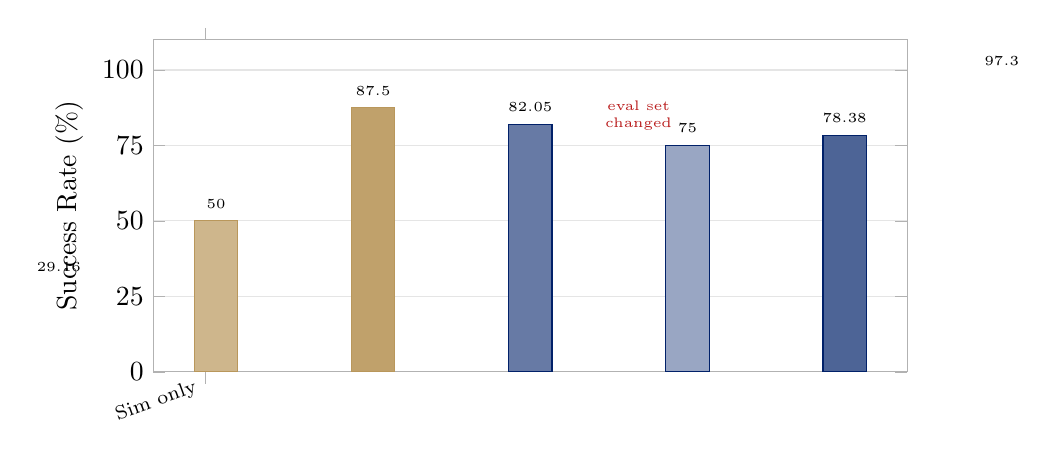
\begin{tikzpicture}
\begin{axis}[
  ybar,
  width=0.92\textwidth,
  height=5.8cm,
  bar width=0.55cm,
  ymin=0, ymax=110,
  ylabel={Success Rate (\%)},
  symbolic x coords={Sim only, +Sim2Real, +Real 2.5h, 1st eval, 2nd eval, 3rd eval, Final},
  xtick=data,
  x tick label style={font=\scriptsize, rotate=20, anchor=east},
  ytick={0,25,50,75,100},
  nodes near coords,
  nodes near coords style={font=\tiny, above},
  every node near coord/.append style={yshift=1pt},
  axis line style={draw=gray!60},
  tick style={draw=gray!60},
  ymajorgrids=true,
  grid style={gray!20},
  enlarge x limits=0.08,
]
  \addplot[fill=negativered!80, draw=negativered] coordinates {
    (Sim only, 29.16)
  };
  \addplot[fill=primarygold!70, draw=primarygold] coordinates {
    (+Sim2Real, 50.00)
  };
  \addplot[fill=primarygold!90, draw=primarygold] coordinates {
    (+Real 2.5h, 87.50)
  };
  \addplot[fill=primaryblue!60, draw=primaryblue] coordinates {
    (1st eval, 82.05)
  };
  \addplot[fill=primaryblue!40, draw=primaryblue] coordinates {
    (2nd eval, 75.00)
  };
  \addplot[fill=primaryblue!70, draw=primaryblue] coordinates {
    (3rd eval, 78.38)
  };
  \addplot[fill=positivegreen!80, draw=positivegreen] coordinates {
    (Final, 97.30)
  };
  % Annotation for the dip
  \node[font=\tiny, text=negativered, align=center] at (axis cs:2nd eval, 85) {eval set\\changed};
\end{axis}
\end{tikzpicture}
\end{document}
